\documentclass[11pt]{beamer}

%\usetheme{Copenhagen}
%\usetheme{Warsaw}
%\usetheme{Frankfurt}
%\usetheme{Darmstadt}
%\usetheme{Berlin}
\usetheme{AnnArbor}
\usefonttheme[onlylarge]{structurebold} 
\setbeamerfont*{frametitle}{size=\normalsize,series=\bfseries} 
\setbeamertemplate{bibliography item}[text]
\setbeamertemplate{navigation symbols}{} 
\usepackage[english]{babel} 
\usepackage[latin1]{inputenc} 
\usepackage{times} 
\usepackage[T1]{fontenc}

\usepackage{tikz} 
\usetikzlibrary{arrows} 
\tikzstyle{block}=[draw opacity=0.7,line width=1.4cm]

\usepackage{ltlfonts}

\usepackage{color} 
\usepackage{alltt} 
\newcommand{\hlstd}[1]{\textcolor[rgb]{0,0,0}{#1}} 
\newcommand{\hlnum}[1]{\textcolor[rgb]{0,0,0}{#1}} 
\newcommand{\hlesc}[1]{\textcolor[rgb]{0,0,1}{#1}} 
\newcommand{\hlstr}[1]{\textcolor[rgb]{0,0,1}{#1}} 
\newcommand{\hldstr}[1]{\textcolor[rgb]{0.5,0.62,0.75}{#1}} 
\newcommand{\hlslc}[1]{\textcolor[rgb]{0.18,0.6,0.34}{#1}} 
\newcommand{\hlcom}[1]{\textcolor[rgb]{0.44,0.48,0.7}{#1}} 
\newcommand{\hldir}[1]{\textcolor[rgb]{0.25,0.37,0.75}{#1}} 
\newcommand{\hlsym}[1]{\textcolor[rgb]{0,0,0}{#1}} 
\newcommand{\hlsymb}[1]{\textcolor[rgb]{1.0,0,0}{#1}} 
\newcommand{\hlline}[1]{\textcolor[rgb]{0,0,0}{#1}} 
\newcommand{\hlkwa}[1]{\textcolor[rgb]{0.5,0,0.33}{\bf{#1}}} 
\newcommand{\hlkwb}[1]{\textcolor[rgb]{0.5,0,0.33}{\bf{#1}}} 
\newcommand{\hlkwc}[1]{\textcolor[rgb]{0.5,0,0.33}{\bf{#1}}} 
\newcommand{\hlkwd}[1]{\textcolor[rgb]{0,0,0}{#1}} 
\definecolor{bgcolor}{rgb}{1,1,1}

\title{Synthesizing Multi-View Models of Software Systems} 
\author{Lambeau Bernard} 
\institute{UCL/EPL/INGI} 
\date{march 2011}

\begin{document}

\begin{frame}
    \titlepage
\end{frame}

\begin{frame}{Outline}
	\small
	\tableofcontents
\end{frame} 

\section{Introduction} 

\begin{frame}{Introduction} 
\end{frame}


\section{A multi-view modeling framework} 

\begin{frame}{A multi-view modeling framework} 
  \begin{block}{Abstract}
    Acts as a background chapter about the models we use, their syntax and semantics. 
    Contributions shared with Damas thesis.
  \end{block}
  \begin{block}{Outline}
    \begin{itemize}
      \item Event-based Behavior Models
        \begin{itemize}
          \item Message Sequence Charts (MSC) for instance behaviors 
          \item Labeled Transition Systems (LTS) for class behaviors
        \end{itemize}
      \item State-based abstractions
        \begin{itemize}
          \item Capturing state information with Fluents
          \item Guards in behavior models
          \item Decorations on behavior models
        \end{itemize}
      \item Intentional models as goal graphs on fluents
        \begin{itemize}
          \item Goals and Fluent Linear Temporal Logic (FLTL)
          \item Linking FLTL and LTS: property and tester automata
        \end{itemize}
    \end{itemize}
  \end{block}
\end{frame}

\begin{frame}{Message Sequence Charts for instance behaviors}
  \begin{center}
	  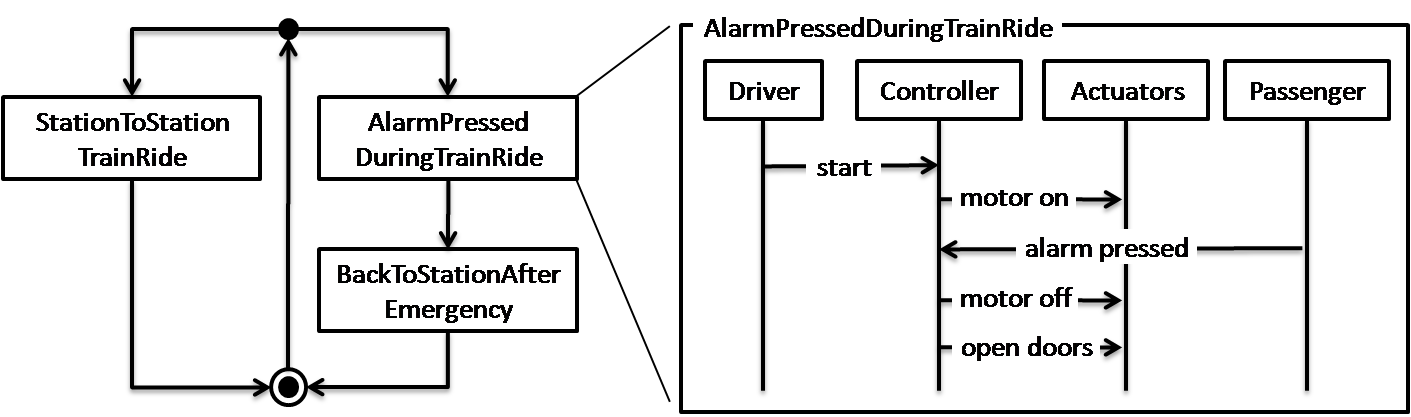
\includegraphics[width=12cm]{images/Train_hMSC_MSC.png}
  \end{center}
  \begin{block}{MSC (right) and high-level MSC (left)}
	  \begin{itemize}
		  \item Syntax of MSC and hMSC is described in \cite{ITU96}
		  \item Semantics of MSC and hMSC is defined in terms of Labeled Transition Systems, following \cite{Uchitel03}
		  \item We also allow a hMSC node to be refined as a finer-grained hMSC
	  \end{itemize}
  \end{block}
\end{frame}

\begin{frame}{Labeled Transition Systems for class behaviors}
  \vspace{-0.5cm}
  \begin{center}
	  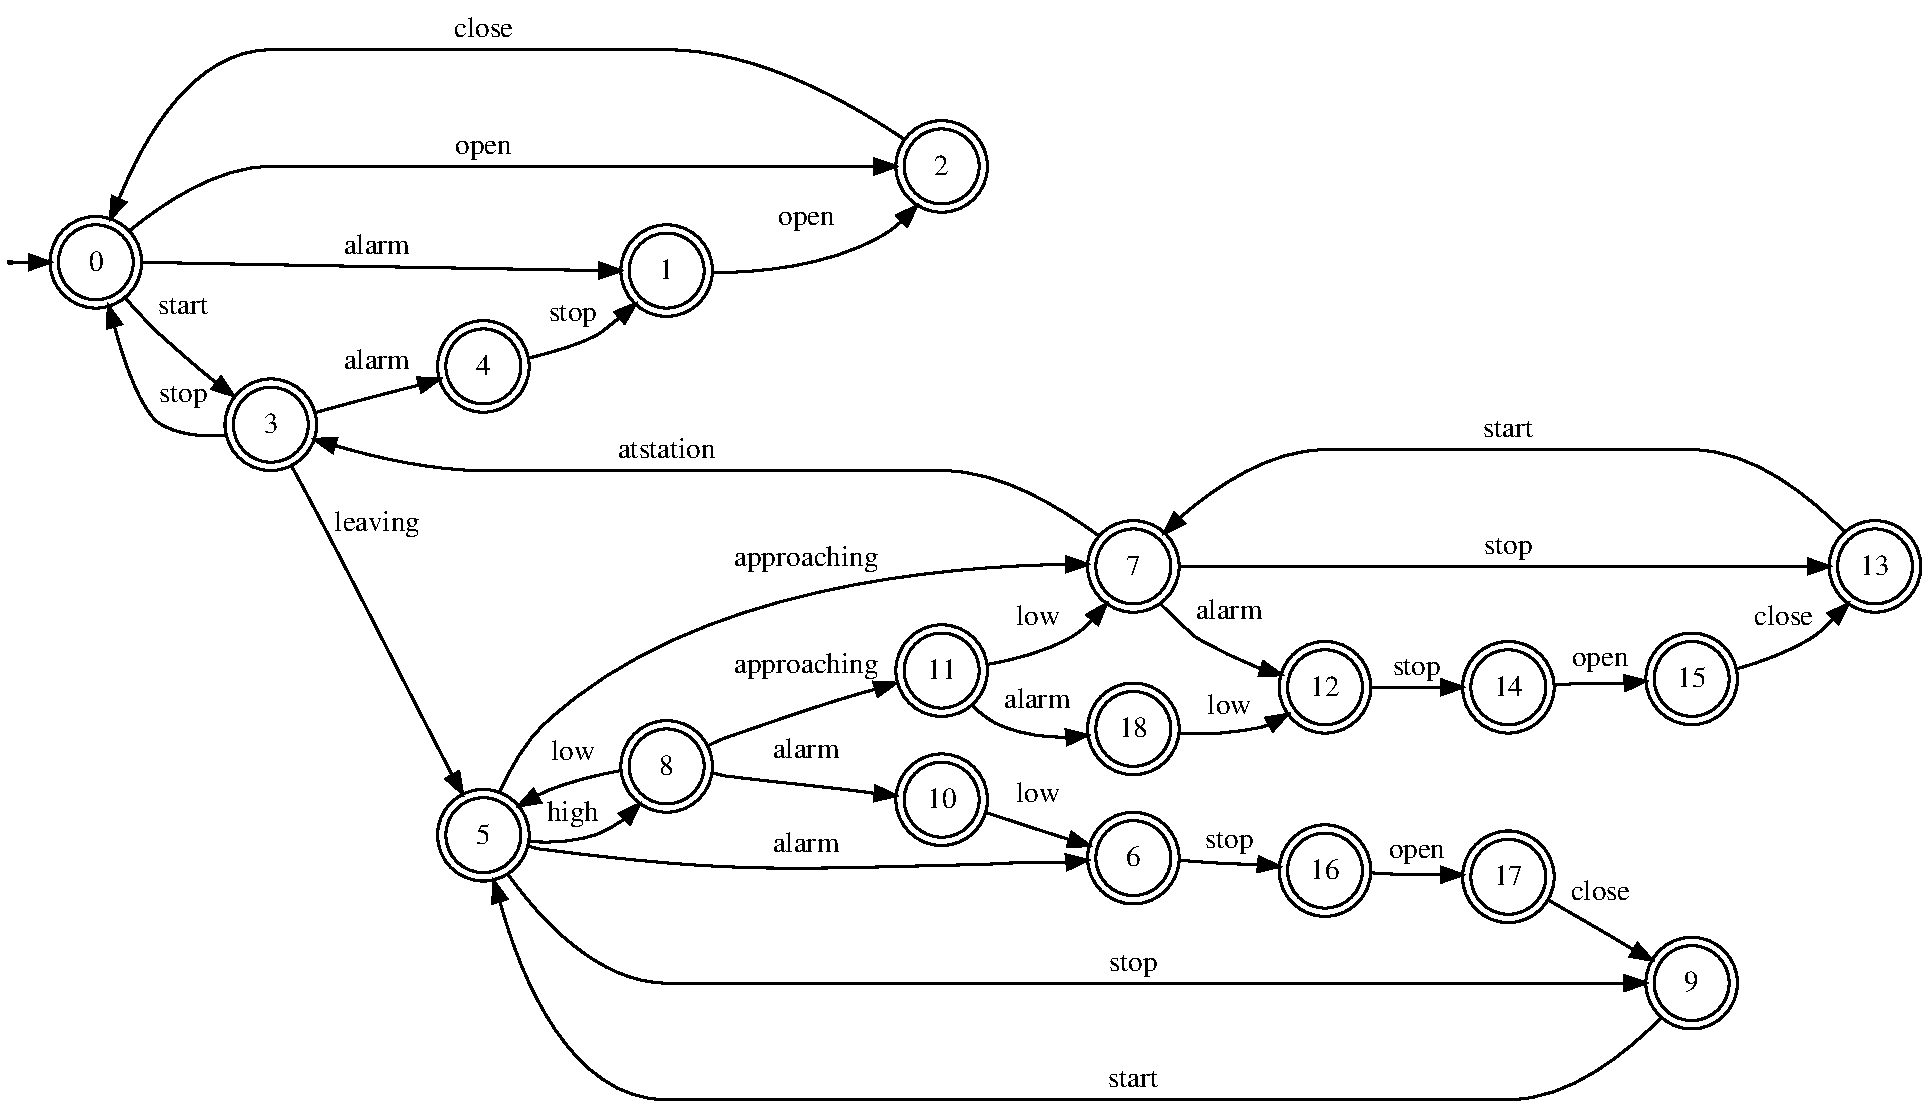
\includegraphics[width=10cm]{images/bigtrain.pdf}
  \end{center}
  \vspace{-1.5cm}
  \begin{block}{Labeled Transition Systems}
	  \begin{itemize}
		  \item Syntax and Semantics defined in \cite{Magee99}
		  \item Each agent behavior is defined by a LTS. The system behavior is defined by LTS composition
		  \item MSCs are admissible traces in the system LTS \cite{Uchitel03}
	  \end{itemize}
  \end{block}
\end{frame}

\begin{frame}{Capturing state information with Fluents}
  \begin{block}{Fluents capture the system state through the occurrence of events \cite{Milner89}}
	  \begin{center}
		  $fluent\;Fl = <init_{Fl}, term_{Fl}> initially\;Init_{Fl}$
	  \end{center}
	  \vspace{-0.4cm}
	  where $init_{Fl}$ and $term_{Fl}$ are disjoint set of events rendering the fluent $true$ and $false$, respectively
  \end{block}
  \begin{block}{Example}
	  \small
	  $fluent\;moving = <start, \{stop, emergency\;stop\}> initially\;false$
	  $fluent\;doors\_closed = <close, \{open, emergency\;open\}> initially\;true$
  \end{block}
\end{frame}

\begin{frame}{Guards in Behavior Models}
  \small
  \begin{block}{Summary}
	  Guards can be formally used in hMSC and LTS, leading to guarded hMSC (g-hMSC) and guarded LTS (g-LTS)
	  \begin{itemize}
	         \item A guard is a boolean expression on fluents
	         \item Structured forms for hMSC and LTS, avoiding state/trace explosion
	         \item Relax the assumption of fluent initial values being known for all instances
	  \end{itemize}
  \end{block}
  \begin{block}{Related publication}
	  \scriptsize
	  Damas C., Lambeau B., Roucoux F. and van Lamsweerde A., \emph{Analyzing Critical Process Models through Behavior Model Synthesis},
	  in Proc. ICSE'2009: 31th International Conference on Software Engineering, Vancouver, Canada, May 16-24, 2009. 
  \end{block}
\end{frame}

\begin{frame}{Guards in hMSC, i.e. g-hMSC}
  \begin{columns}
	  \column{.5\textwidth}
		  \begin{block}{Summary}
			  \begin{itemize}
				  \item \emph{Decision nodes}: outgoing transitions are labeled by boolean expressions on fluents
				  \item Initial condition $C_0$ stating an invariant on the initial state
				  \item Trace semantics through guarded LTS and LTS
				  \item Automated checking of guards: \emph{non overlapping}, \emph{completeness} and \emph{reachability}
			  \end{itemize}
		  \end{block}
	  \column{.5\textwidth}
		  \begin{center} 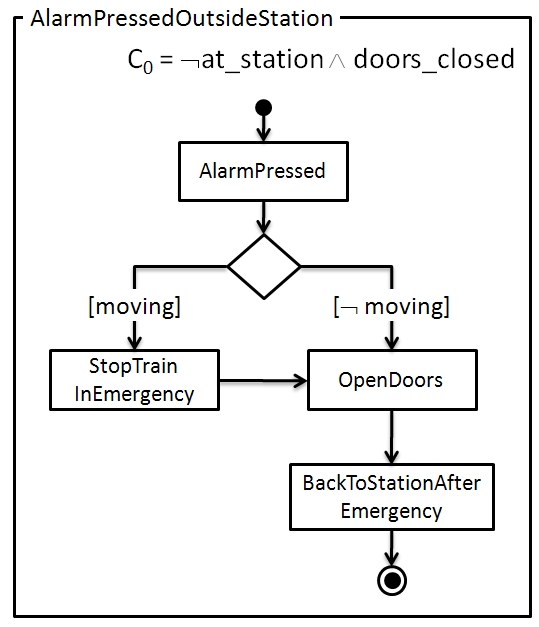
\includegraphics[width=5.5cm]{images/Train_guarded_hMSC.jpg} \end{center}
  \end{columns}
\end{frame}

\begin{frame}{Guards in LTS, i.e. g-LTS}
  \begin{block}{Summary}
	  \begin{itemize}
		  \item A g-LTS transition is labeled by an event or a guard
		  \item Initial condition $C_0$ stating an invariant on the initial state
		  \item A trace is accepted by a g-LTS if three conditions hold: \emph{trace inclusion}, \emph{admissible start} and \emph{guard satisfaction}
	  \end{itemize}
  \end{block}
  \begin{block}{Example}
	  \begin{center} 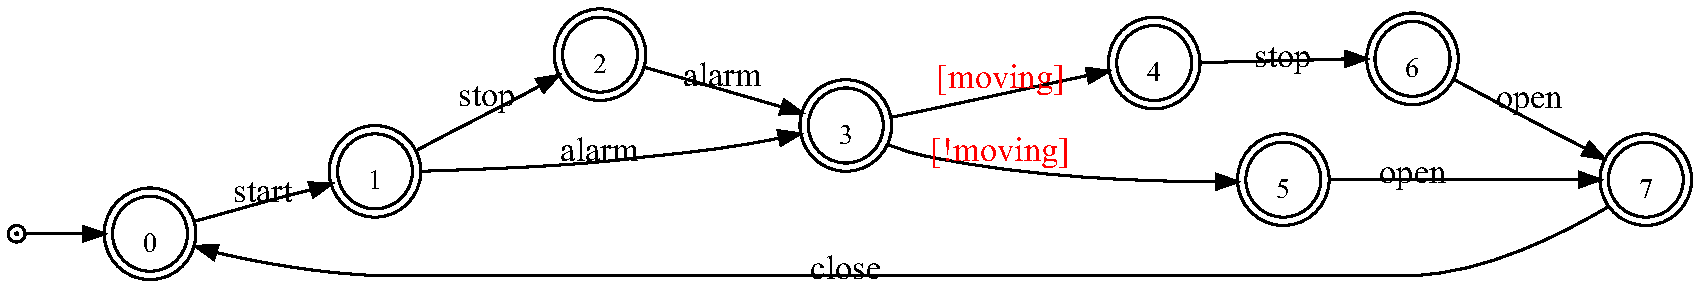
\includegraphics[width=11cm]{images/Train_guarded_LTS.pdf} \end{center}
	  \vspace{-0.5cm}
	  \begin{itemize}
		  \item $C_0 = \neg moving \wedge doors\_closed$
		  \item The event trace $(start\;alarm\;open)$ is not accepted due to the \emph{guard satisfaction} condition
	  \end{itemize}
  \end{block}
\end{frame}


\section{Deductive synthesis of LTS models from guarded hMSCs}

\begin{frame}{Deductive synthesis of LTS models from guarded hMSCs}
  \begin{block}{Chapter Outline}
    \begin{itemize}
      \item From guarded hMSC to guarded LTS
      \item From guarded LTS to pure LTS
      \item Model analysis perspectives of deductive synthesis
    \end{itemize}
  \end{block}
\end{frame}



\section{References}
\begin{frame}[allowframebreaks]{References}
	\tiny
	\bibliographystyle{alpha}
	\bibliography{slides} 
\end{frame}

\end{document}
